\documentclass{article}\usepackage[]{graphicx}\usepackage[]{color}
%% maxwidth is the original width if it is less than linewidth
%% otherwise use linewidth (to make sure the graphics do not exceed the margin)
\makeatletter
\def\maxwidth{ %
  \ifdim\Gin@nat@width>\linewidth
    \linewidth
  \else
    \Gin@nat@width
  \fi
}
\makeatother

\definecolor{fgcolor}{rgb}{0.345, 0.345, 0.345}
\newcommand{\hlnum}[1]{\textcolor[rgb]{0.686,0.059,0.569}{#1}}%
\newcommand{\hlstr}[1]{\textcolor[rgb]{0.192,0.494,0.8}{#1}}%
\newcommand{\hlcom}[1]{\textcolor[rgb]{0.678,0.584,0.686}{\textit{#1}}}%
\newcommand{\hlopt}[1]{\textcolor[rgb]{0,0,0}{#1}}%
\newcommand{\hlstd}[1]{\textcolor[rgb]{0.345,0.345,0.345}{#1}}%
\newcommand{\hlkwa}[1]{\textcolor[rgb]{0.161,0.373,0.58}{\textbf{#1}}}%
\newcommand{\hlkwb}[1]{\textcolor[rgb]{0.69,0.353,0.396}{#1}}%
\newcommand{\hlkwc}[1]{\textcolor[rgb]{0.333,0.667,0.333}{#1}}%
\newcommand{\hlkwd}[1]{\textcolor[rgb]{0.737,0.353,0.396}{\textbf{#1}}}%

\usepackage{framed}
\makeatletter
\newenvironment{kframe}{%
 \def\at@end@of@kframe{}%
 \ifinner\ifhmode%
  \def\at@end@of@kframe{\end{minipage}}%
  \begin{minipage}{\columnwidth}%
 \fi\fi%
 \def\FrameCommand##1{\hskip\@totalleftmargin \hskip-\fboxsep
 \colorbox{shadecolor}{##1}\hskip-\fboxsep
     % There is no \\@totalrightmargin, so:
     \hskip-\linewidth \hskip-\@totalleftmargin \hskip\columnwidth}%
 \MakeFramed {\advance\hsize-\width
   \@totalleftmargin\z@ \linewidth\hsize
   \@setminipage}}%
 {\par\unskip\endMakeFramed%
 \at@end@of@kframe}
\makeatother

\definecolor{shadecolor}{rgb}{.97, .97, .97}
\definecolor{messagecolor}{rgb}{0, 0, 0}
\definecolor{warningcolor}{rgb}{1, 0, 1}
\definecolor{errorcolor}{rgb}{1, 0, 0}
\newenvironment{knitrout}{}{} % an empty environment to be redefined in TeX

\usepackage{alltt}
\usepackage[hidelinks]{hyperref}
\usepackage[style=authoryear,backend=bibtex8]{biblatex}
\usepackage[utf8]{inputenc}
\addbibresource{library.bib}
\usepackage[capposition=top]{floatrow}
\usepackage{xesearch}
\newcounter{words}
\newenvironment{counted}{%
\setcounter{words}{0}
\SearchList!{wordcount}{\stepcounter{words}}
{a?,b?,c?,d?,e?,f?,g?,h?,i?,j?,k?,l?,m?,
n?,o?,p?,q?,r?,s?,t?,u?,v?,w?,x?,y?,z?}
\UndoBoundary{'}
\SearchOrder{p;}}{%
\StopSearching}

\usepackage{amsmath}
\IfFileExists{upquote.sty}{\usepackage{upquote}}{}
\begin{document}

\title{Reviving the Labor Market Competition Hypothesis of Anti-Immigrant Attitudes? Experimental Evidence from a Nationally Representative Sample}
\author{Jonathan Mellon}
\date{\today}

\maketitle
\begin{counted}


%context

Western democracies have seen a substantial rise in the salience of immigration in the last decade, a trend which has resulted in increased success for radical right parties and candidates across these countries  \cite{Akkerman2012,Dahlstrom2012,Mudde2013,Abou-Chadi2015}. However, the causes of anti-immigrant sentiment are strongly contested within political science. On the one hand, descriptive work has tended to find that economic concerns strongly correlate with anti-immigrant sentiment \autocite{Mayda2006,Dancygier2013,Malhotra2013,Helbling2011,Ford2014}, particularly in terms of native workers' perception that they are being economically threatened by migrants. On the other hand, experimental work has found that anti-immigrant sentiment does not appear to reflect the predictions of economic theory, which would suggest that native workers will be most threatened by immigrants with skill levels similar to their own \autocite{Hainmueller2007,Hainmueller2010,Bohrer2013,Harell2012, Goldstein2014,Hainmueller2015}.


%%%% Research question
This article argues that these experimental tests of labor market threat do not test threat in a way that is equivalent for high and low skilled workers because a much smaller proportion of high skilled immigrants threaten high skilled natives compared to the threat of low skilled immigrants to low skilled natives. Low skilled jobs are relatively unprotected from competition, because anyone can potentially do that job. By contrast, high skilled workers are protected from almost all competition except from people with precisely the same set of skills as them.


To deal with this asymmetry,I use a novel experimental test of the labor market competition hypothesis by presenting a random subset of subjects on a nationally representative survey with potential immigrants who would work in the same occupation as the subject, thereby testing the effect of immigrants who are directly competing with the respondent economically.

%%%% Findings
I find strong evidence for the labor market competition hypothesis. While respondents prefer high skilled to low skilled immigrants in general, they are as opposed to immigrants who directly compete with them as they are to low skilled immigrants. This effect holds both for low and high skilled natives, showing that labor market competition can generate anti-immigrant attitudes even in high skilled natives. Additional analysis finds that low skilled natives feel economically threatened both by generic low skilled immigrants, whereas high skilled natives do not feel economically threatened by generic high skilled immigrants.

%%%% Academic implications of findings
These results help to resolve the divide between observational and experimental research and suggest that the field has been too quick to dismiss the economic dimension of anti-immigrant attitudes. These results instead suggest that there are multiple reasons why people may oppose immigration.

%%% more here


%%%% Wider implications of findings



%%%% Robustness

% Mechanism testing

% replicating previous findings



%%%% wider wider implications
These findings also have implications for policy. If anti-immigrant attitudes were purely cultural, then addressing any economic effects of immigration would be ineffective in increasing support for immigration. While these results certainly do not dismiss the role that cultural factors play in anti-immigrant sentiment, policymakers should perhaps be less quick to dismiss economic concerns as automatically being cover for cultural fears. 



\section{The Labor Market Competition Hypothesis of Anti-immigration Attitudes}

Perceived labor market competition has been heavily contested as a cause of anti-immigrant sentiment. The evidence has been unusually divided, with observational studies finding mixed evidence for the link and experimental evidence finding no effect. 

One line of observational evidence for the effect of perceived economic competition on anti-immigrant attitudes comes from the strong relationship between educational attainment and pro-immigrant attitudes \autocite{Scheve2001,Mayda2006}. Other observational work has pointed to evidence that workers in growing industries are more pro-immigration than workers in shrinking industries \autocite{Dancygier2013}, that technology workers oppose H1B visas (which Indian technology workers often immigrate on) but not Indian immigration more generally \autocite{Malhotra2013}, and that high skilled Swiss workers who are early in their careers oppose German immigration \autocite{Helbling2011}. On the other hand, \textcite{Facchini2013} find no evidence of labor market competition effects in South Africa and \textcite{Dustmann2007} find only a weak relationship in the United Kingdom.

The existing experimental evidence almost entirely points against the labor market competition hypothesis, consistently finding that labor market competition is not a cause of anti-immigrant attitudes. \textcite{Hainmueller2010} pioneered the approach of randomly assigning the skill level of hypothetical immigrants to assess whether native workers were more negative towards immigrants of the same skill level as them. Studies following this approach have consistently found that both high and low skilled native workers prefer high to low skilled immigrants \autocite{Hainmueller2007, Hainmueller2010, Bohrer2013, Harell2012, Goldstein2014, Hainmueller2015} Since the labor market competition theory predicts that workers should be most opposed to immigrants with similar skills to them, this has been interpreted as decisive evidence against the labor market competition theory. Instead this line of research has tended to argue that cultural factors are the key factor in explaining anti-immigrant sentiment. 

While previous experimental approaches are a large improvement on studies which conclude that labor market competition is important simply because pro-immigration attitudes correlate with educational attainment, they still constitute an imprecise test of the labor market competition hypothesis. The main reason for this is that a generic “low skilled” immigrant is genuinely a more realistic economic threat to a low skilled native than a generic “high skilled” immigrant is to a high skilled native. This is because high skilled occupations have much more specific human capital requirements than low skilled occupations. An influx of foreign dentists poses essentially zero economic threat to native software developers. By contrast, an influx of foreign care workers could easily threaten the jobs of low skilled native workers in other low skilled occupations such as cleaners and servers, as there is relatively little difference in the requirements of each job. This also fits with the economic literature’s findings that immigration differentially lowers the wages and employment of certain workers (generally low-skilled in the United States and British context), while benefiting others \autocite{Borjas2003,Peri2009,Orrenius2007}, although most studies have found even these effects to be relatively modest \autocite{Peri2009,Ottaviano2012,Gaston2013}.

Given that the economic threat in previous experiments may not be equal across different native skill levels, the finding that all natives prefer high to low skilled immigration may instead reflect the expected benefit of different immigration. With the exception of doctors themselves, both high and low skilled natives will likely benefit more from a greater supply of physicians than they will from a greater supply of fruit pickers, while the economic costs in terms of government benefits, housing competition etc are likely to remain relatively similar across different immigrant skill levels. 

A fairer test of the labor market hypothesis theory therefore requires a treatment that could be as economically competitive for high skilled workers as it is for low skilled workers, rather than simply relying on generic high or low skilled labels.


%%% more economics in this section





\section{Experimental Design, Data, Model Specification, and Analysis}

This paper builds on the existing experimental designs that test labor market competition by presenting different types of immigrants to a survey respondent. The key difference in my approach is that respondents are asked whether they would favor more immigrants in particular occupations. As well as being randomly assigned immigrants from a set of pre-defined high and low skilled occupations, I also assign half of the subjects to be asked about immigrants who would be looking for work in the same occupation as the respondent (which was collected in a previous survey wave), which is the key labor market competition treatment in this paper. Finally, two jobs are included in the prompt in order to make the insertion of the respondent's own job slightly less obvious as well.

\begin{figure}

\includegraphics[width=10cm]{figure/main_experment.png}
\caption{Example of a survey screen that would be seen by a respondent in the experiment.}
\label{fig:experimentScreen}
\end{figure}


To code the occupations of the respondents, I took the open ended occupation responses of 7585 respondents and manually coded a job that would fit into the following question stem:
\begin{quote}
Professors at several leading universities have said that Britain's economy could be greatly improved if more people were allowed to immigrate to Britain for jobs including \$Job1 and \$Job2. Do you agree that \textit{more} people like this should be allowed to \textit{come to Britain} to live and work?
\end{quote}
in the \$Job2 position. Examples include: train drivers, account managers, warehouse workers and teaching assistants. In total, 299 unique jobs were coded in the data. An example of the screen a respondent would see is shown in figure \ref{fig:experimentScreen}. 

The experiment is designed to make the insertion of the respondent's occupation less obvious in several ways. Firstly, I code the occupation text to be as specific as possible, without making it obvious to the respondent that the text is copied from their occupation responses on a previous survey wave. Secondly, the experimental wave was fielded nearly a year after the occupational data was collected to reduce the chance that respondents  explicitly remember having given their occupation. Finally, two jobs are included in the question to make it appear that the respondent's occupation merely happened to be one of the ones mentioned.

For \$Job1, respondents are randomly assigned one of the twelve occupations. The low skill jobs are randomly assigned as one of waiters, drivers, receptionists, shop assistants, carers, and cleaners and the high skill jobs are randomly assigned between senior managers, doctors, lawyers, lecturers, engineers, and programmers.

For \$Job2, half of respondents are assigned their own occupation. The other half of respondents are randomly assigned one of the twelve occupations. If respondents are assigned the same job twice or if one of the jobs happens to be their own job (in the control condition), the job is replaced with another job of the same skill level from the list. The assignments in the limit and in practice are shown in table \ref{table:assignment}. Balance checks on educational level and prior anti-immigrant attitudes are shown in appendix \ref{app:balance_checks} and show no significant differences.


% latex table generated in R 3.2.3 by xtable 1.7-4 package
% Thu May 12 15:55:35 2016
\begin{table}[ht]
\centering
\begin{tabular}{rlllr}
  \hline
 & Assignment & \% in limit & Cases assigned & \% assigned \\ 
  \hline
1 & Low skilled/own occupation & 25 & 1213 & 24.90 \\ 
  2 & High skilled/own occupation & 25 & 1235 & 25.30 \\ 
  3 & Both high skilled & 12.5 & 611 & 12.50 \\ 
  4 & Both low skilled & 12.5 & 655 & 13.40 \\ 
  5 & Low skilled and high skilled & 25 & 1164 & 23.90 \\ 
   \hline
\end{tabular}
\caption{Experimental assignments} 
\label{table:assignment}
\end{table}


The key hypothesis of this paper is that respondents will be less willing to accept immigrants who directly compete with them economically than other immigrants. Given that previous research has already demonstrated that both low and high educated natives dislike low skilled immigrants compared to high skilled immigrants, the key comparison is between the preferences of high skilled natives for high skilled immigrants and high skilled immigrants who would in the same occupation as the respondent. While I hypothesize that both high and low skilled natives will prefer generic high skilled immigrants to immigrants who are a labor market threat, it is not clear from theory whether we should expect native workers to prefer low skilled immigrants or immigrants who are a labor market threat.

In the case of low skilled native workers, any low skilled immigrant is already a potential labor market threat because there are few barriers to entry in low wage labor markets. In the case of high skilled native workers, low skilled migrants are not a labor market threat, but they may be less desirable because they may be seen as increasing demands on the welfare state (increasing taxes) or because they are seen as less culturally desirable \autocite{Hainmueller2015a}.

Additionally, the structure of this experiment allows me to attempt a replication of previous experimental findings that: both low and high skilled natives prefer high to low skilled immigrants and that high skilled natives are more positive towards immigration in general. These hypotheses are only tested within the group of respondents who do not receive the own job experimental assignment.

While the labor market competition hypothesis suggests that the effect of immigrant occupations will be primarily through economic threat, others  argue that particular immigrant occupations can signal cultural threats as well \autocite{Hainmueller2015a}. I test both of these mechanisms by collecting two manipulation check variables testing whether respondents feel economically threatened or culturally threatened.   

The economic threat measures asks ``How worried would you be about \textit{your job prospects} if  immigrants like these were allowed to come to Britain in greater numbers?", with responses recorded on a 1 to 7 scale from ``Not at all worried" to "Very worried". The cultural threat measure asks "How worried would you be about immigrants like these fitting into British society?", with responses recorded on a 1 to 7 scale from "Not at all worried" to "Very worried".

I also break down the experimental results according to the skill level of the respondents. Following previous experimental research on immigrant attitudes \autocite{Hainmueller2015a, Hainmueller2010}, I use educational attainment as a proxy for skill level. I combine the educational attainment of the respondents into three categories: high (undergraduate level qualification or higher), medium (left school at 18 with qualifications such as A-levels), and low (left school with age 16 qualifications such as GCSEs or lower).

All analysis in this paper was pre-registered at the Experiments in Governance and Politics (EGAP) registry except where otherwise noted.\footnote{Link will go here.} The pre-analysis plan consisted of a knitr document that also formed the template for the current paper.

\subsection{Model Specification}

Each of the hypotheses is tested using an ordered logistic regression estimator. For instance hypotheses A and B are tested by predicting the latent variable $y^*$, which is observed as an ordinal variable $y$ which takes values:

\begin{math} y= \begin{cases}
1 & \text{if } y^* \le \mu_1, \\
2 & \text{if } \mu_1<y^* \le \mu_2, \\
3 & \text{if } \mu_2 <y^* \le \mu_3, \\
\vdots \\
7 & \text{if }  y^* > \mu_{7}
\end{cases}\end{math}

The coefficients $ \beta_1... \beta_9$ are estimated using maximum likelihood estimation:
\begin{multline}
y^* =  \beta_1 low_{j1} + \beta_2 low_{j2} + \beta_3 own_{j2} + \beta_4 educ_{low} + 
\beta_5 educ_{med} + 
\beta_6 educ_{low} * own_{j2} + \\
\beta_7 educ_{med} * own_{j2} + 
\beta_8 educ_{low} * low_{j2} + 
\beta_9 educ_{med} * low_{j2} \\
\end{multline}
, where $low_j1$ refers to a low skilled job in the job 1 position, $own_{j2}$ refers to the respondent's own job in the job 2 posiition and $educ_{low}$ is a dummy capturing whether a respondent is in the low educational attainment category.

\subsection{Sample}

The experiment was fielded in wave 7 (April 2016) of the British Election Study Internet Panel to 4878 respondents (around a quarter of the sample excluding topup respondents and respondents whose occupation could not be coded on a previous wave).\footnote{The experiment is covered by the British Election Study's ethical clearance from the University of Manchester, which explicitly includes survey experiments.} The survey was only fielded to respondents who had taken a previous wave of the British Election Study and had given a current or   recent occupation that could be coded for the experiment. The time period of the fieldwork was directly prior to the devolved and local elections around the UK and two months prior to the referendum on Britain's membership of the European Union, where immigration is a highly salient issue. The fieldwork for the British Election Study Internet Panel is conducted online by YouGov and is quota sampled and weighted to be politically and demographically representative of the British population. While the sample is not a true probability sample, previous work has found Internet panels to be consistent in their correlation structures \autocite{Sanders2007}, although not always correct on the exact univariate distributions of variables \autocite{Mellon2016}. Given that this study is experimental and that previous experimental studies have found consistent results across different contexts, the level of representativeness is sufficient to be confident of the external validity of these experimental results. The full syntax for the experiment is shown in appendix \ref{appendix:experimentsyntax}.

\section{Effects of Labor Market Competition on Support for Greater Immigration}


\begin{table}
\begin{center}
\begin{tabular}{l c }
\hline
 & Model 1 \\
\hline
Low education              & $-1.22^{***}$ \\
                           & $(0.12)$      \\
Medium education           & $-0.74^{***}$ \\
                           & $(0.14)$      \\
Job 1: low skill           & $-0.62^{***}$ \\
                           & $(0.05)$      \\
Job 2: Low skill           & $-0.40^{***}$ \\
                           & $(0.12)$      \\
Job 2: own job             & $-0.34^{***}$ \\
                           & $(0.10)$      \\
Low ed. * low skill job    & $-0.06$       \\
                           & $(0.17)$      \\
Medium ed. * low skill job & $0.00$        \\
                           & $(0.20)$      \\
Low ed. * own job          & $-0.23$       \\
                           & $(0.15)$      \\
Medium ed. * own job       & $-0.15$       \\
                           & $(0.17)$      \\
\hline
AIC                        & 16191.94      \\
BIC                        & 16287.95      \\
Log Likelihood             & -8080.97      \\
Deviance                   & 16161.94      \\
Num. obs.                  & 4449          \\
\hline
\multicolumn{2}{l}{\scriptsize{$^{***}p<0.001$, $^{**}p<0.01$, $^*p<0.05$}}
\end{tabular}
\caption{Ordered logistic regression predicting acceptance of immigrants. (Reference categories: high education, Job 1: high, skill, and Job 2: high skill)}
\label{table:mainLabMarket}
\end{center}
\end{table}



\begin{figure}
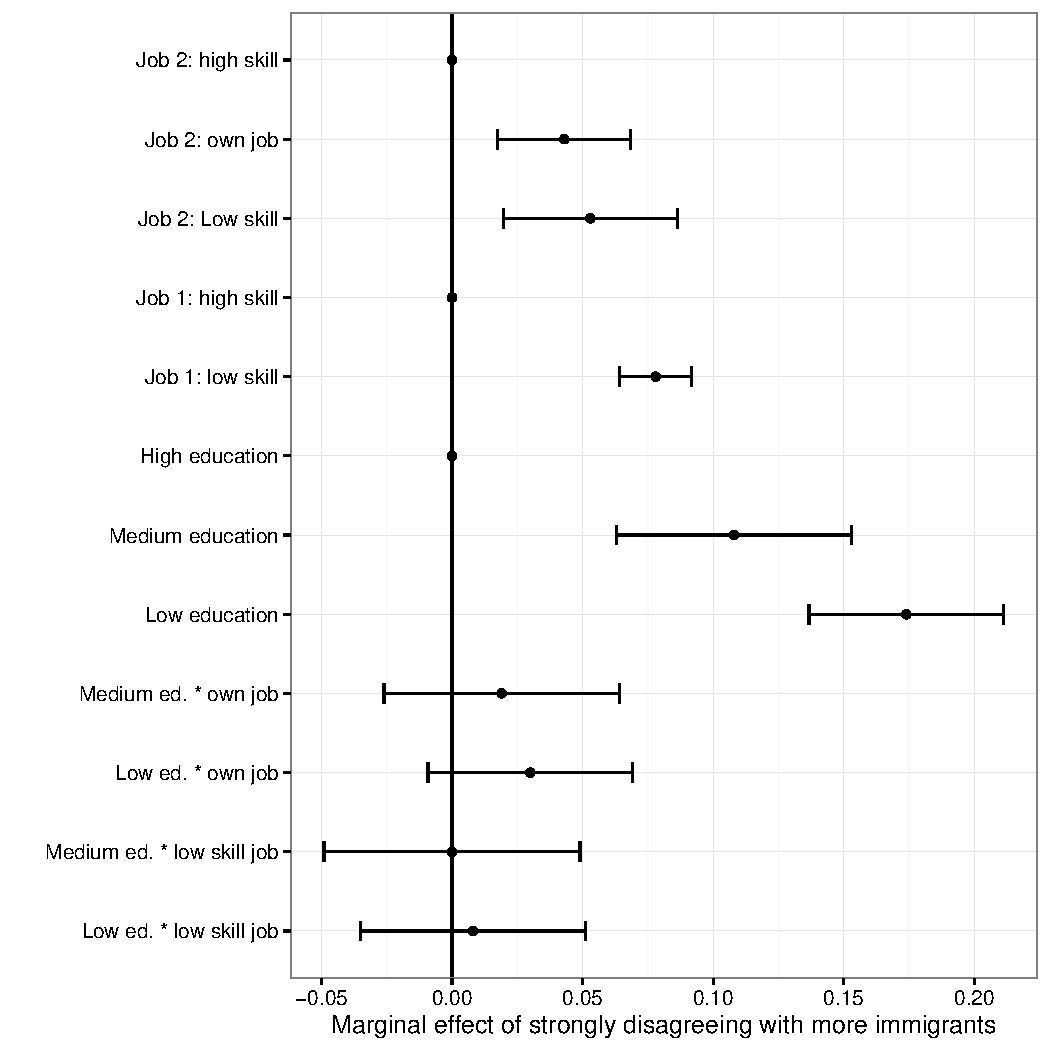
\includegraphics[width=\maxwidth]{figure/mainLabMarketMFX-1} \caption[Effects of labor market competition treatment on probability of `strongly disagreeing' that more immigrants should be allowed to come to Britain]{Effects of labor market competition treatment on probability of `strongly disagreeing' that more immigrants should be allowed to come to Britain}\label{fig:mainLabMarketMFX}
\end{figure}




Figure \ref{fig:mainLabMarketMFX} shows the marginal effects of the experimental conditions on the probability of choosing the ``strongly disagree'' (1 on the 1-7 scale) of whether more immigrants should be allowed to live in Britain. The marginal effects are indicated by dots and the lines show the 95\% confidence intervals. The dots with no lines are the reference categories for categorical variables. The full regression table is shown in Table \ref{table:mainLabMarket}. The results show that subjects presented with their own job are 4.3 percentage points more likely to say that they ``strongly disagree'' that more immigrants should be allowed to come to Britain. The magnitude of this effect is almost exactly the same as the effect of being presented with the 5.3 percentage point effect (SE=1.7) of presenting a 4.3 percentage point effect (SE=1.3) of presenting a low skilled immigrant in the second slot.

The model includes high skilled natives and high skilled immigrants as the base categories, so this effect should be interpreted as the comparison between the preference for a generic high skilled immigrant and a high skilled immigrant who is directly competing with the high skilled native respondent. 

Table \ref{table:manipulation_checks} shows that the own job treatment does seem to be succeeding in making respondents more worried about their job prospects if more immigrants were allowed to come to Britain, but that it does not significantly predict cultural threat. This suggests that the effect of the stated occupation is primarily an economic rather than cultural one. 

Table \ref{table:mainLabMarket} also shows the interactions between native skill levels and the treatment effects. None of the interactions are significant or substantial indicating that the treatment effect of labor competition is relatively stable across skill levels.


\begin{table}
\begin{center}
\begin{tabular}{l c c }
\hline
 & Job prospects & Cultural threat \\
\hline
Treatment      & $0.22^{***}$ & $0.07$   \\
               & $(0.05)$     & $(0.05)$ \\
\hline
AIC            & 15656.96     & 17260.73 \\
BIC            & 15701.64     & 17305.66 \\
Log Likelihood & -7821.48     & -8623.36 \\
Deviance       & 15642.96     & 17246.73 \\
Num. obs.      & 4374         & 4533     \\
\hline
\multicolumn{3}{l}{\scriptsize{$^{***}p<0.001$, $^{**}p<0.01$, $^*p<0.05$}}
\end{tabular}
\caption{Manipulation checks. Ordered logistic regression predicting worry about job prospects.}
\label{table:manipulation_checks}
\end{center}
\end{table}


\subsection{Why have previous studies not found evidence of labor market competition?}

Given the strong effect of labor market competition in this experiment, an important question is why previous studies have found null effects. The design of the experiment in this paper makes it possible to look at whether the results which have previously been intepreted as refuting the labor market competition hypothesis replicate in this study. 

The control group in this study also allows me to run a replication of previous experimental studies of anti-immigrant attitudes. The original \textcite{Hainmueller2010} experiment describes the immigrants simply as low or high skilled. While the experiment does not say this explicitly, it would be easy to read the question as simply about whether the immigrants are good or bad at their jobs i.e. you could have a low skilled dentist or a high skilled waiter. The experiment in this paper, sidesteps this issue by using a range of actual jobs of immigrants. 
Followup studies have used particular low and high skilled occupations in a similar approach to this experiment, and found similar results. 

Figure \ref{fig:mainReplication} shows the marginal effects from an ordered logistic regression predicting support for allowing more of a particular type of immigrant into Britain. The regression is run only on the 2430 respondents who did not receive their own job in the the manipulations within the control group (who were not shown their own occupation). The results entirely replicate the findings of the previous studies showing that less skilled natives are consistently less favorable towards immigration and that both high and low skilled natives prefer high to low skilled immigrants.

These findings suggest that previous studies are correct in their findings that native workers from all skill levels prefer high to low skilled immigration. However, given the overall labor competition finding, it appears that generic high and low skilled immigrants do not reliably generate economic threat to natives with similar skill levels.

Figure \ref{fig:manipCheckCompete} shows the effects of the low and high skilled treatments excluding the ``own job'' treatment group on the probability of a respondent saying that they would be ``not at all worried'' about their job prospects if more of these immigrants came to Britain. The results show that there is not a significant main effect of the low skilled treatment group, but that there is a significant negative interaction between low education respondents and the low skilled treatment group. Since high education respondents are the base cateogry, this means that low skilled respondents are economically threatened by the low skill treatment, but that there is not a significant effect on highly educated respondents of the high skill treatment. In other words, the previous immigation experiments appear to only have been treating the lower educated section of their sample with a labor market competition treatment.

\begin{figure}
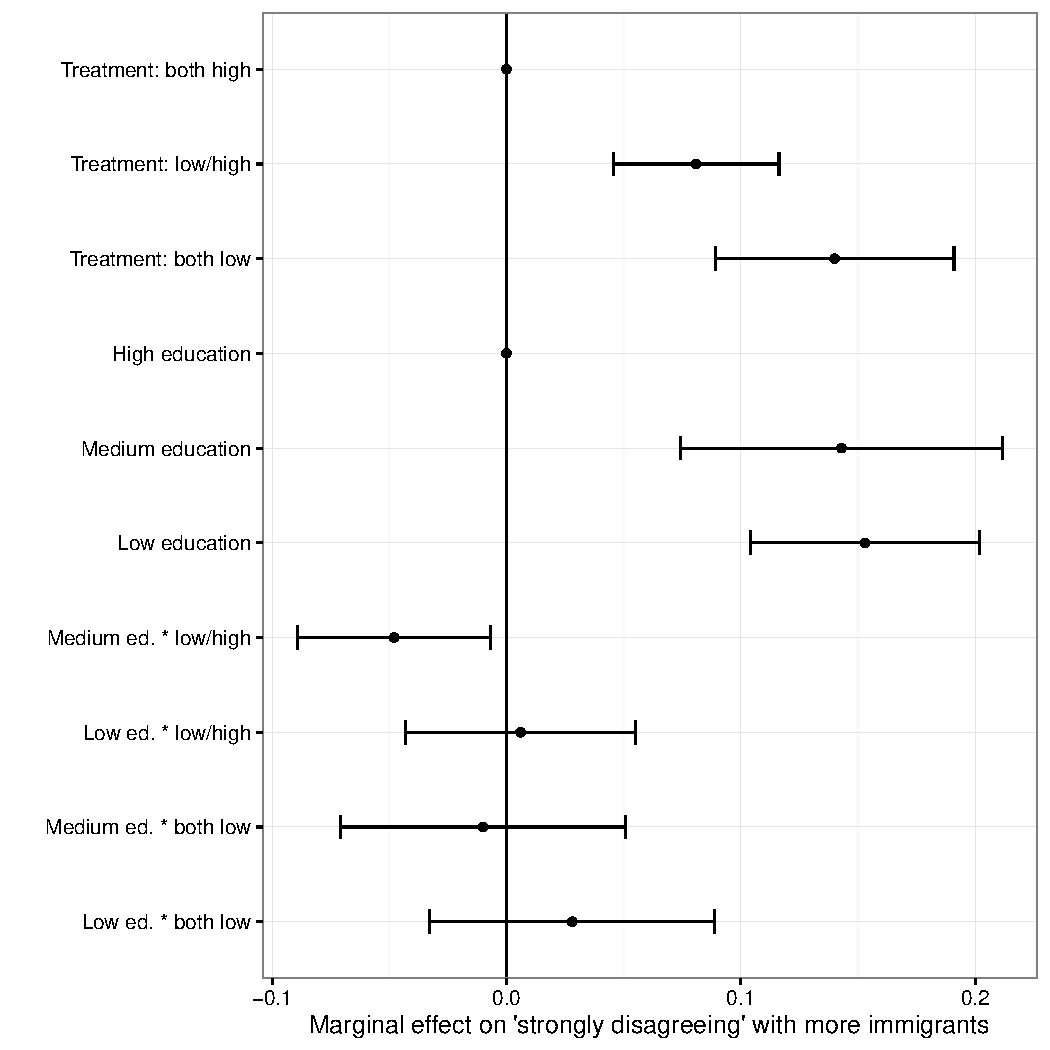
\includegraphics[width=\maxwidth]{figure/mainReplication-1} \caption[Effects of immigrant skill levels on probability of `strongly disagreeing' that more immigrants should be allowed to come to Britain (excludes `own job' treatment group)]{Effects of immigrant skill levels on probability of `strongly disagreeing' that more immigrants should be allowed to come to Britain (excludes `own job' treatment group)}\label{fig:mainReplication}
\end{figure}




\begin{figure}
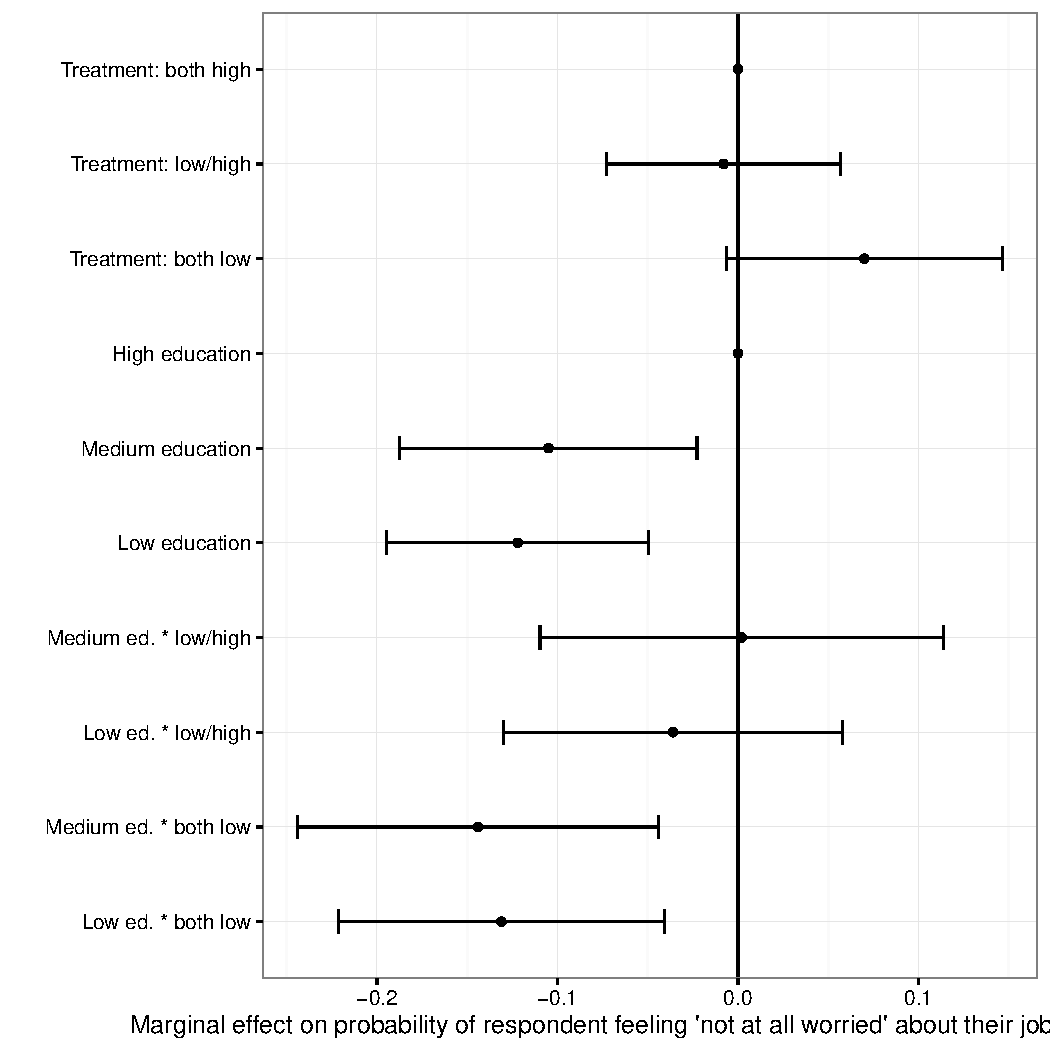
\includegraphics[width=\maxwidth]{figure/manipCheckCompete-1} \caption[Effects of education and immigrant skill level on probability of respondent being `not at all worried' about their own job prospects (excludes `own job' treatment group)]{Effects of education and immigrant skill level on probability of respondent being `not at all worried' about their own job prospects (excludes `own job' treatment group)}\label{fig:manipCheckCompete}
\end{figure}




\section{Discussion and Conclusion}

This article helps to reconcile the previous conflict between observational and experimental evidence about the effect of labor market competition on anti-immigrant attitudes. Previous experimental evidence relied on a relatively undifferentiated measure of labor market competition: whether native workers and immigrants are high or low skilled. Recent observational work, by contrast, argued that labor market competition was an important but not a prevalent factor in anti-immigrant attitudes. This study provides an experimental analysis that corroborates the observational results, while explaining the previous experimental findings. 

The evidence presented here does not prove that cultural threat plays no role in anti-immigrant attitudes. Even when using a direct manipulation of competition, higher skilled natives are still more positive towards immigrants than low skilled natives. However, if a single sentence can reduce support for high skilled immigrants to the level of support for low skilled immigrants, it suggests that higher educated workers' support for immigration may not be as robust as previously believed. Low skilled workers are always potentially under economic threat, as there is generally little protection from competition due to the low barriers to entry. Consequently, low skilled workers are likely to be socialised in an environment that makes them more acutely aware of labor market competition and immigration's potential economic threat. 

Although previous research has suggested that labor market competition is not a prevalent cause of anti-immigrant sentiment, the findings here would suggest that it can play a substantial role. Further research is needed to understand exactly how large a role that practice. However, given that the group that is generally the most anti-immigrant is also the group that will be most economically threatened by immigrants in the real world, there is certainly the possibility that perceived labor market competition may be a substantial driver of anti-immigrant attitudes in Western countries.

The results here are of course only a single study in a single country context. However, given that the experiment in this paper also replicates the key finding that native workers of all skill levels prefer high to low skilled immigrants and that more educated respondents are more likely to support more immigration, it is highly plausible that these results will generalize to other country contexts. Future research should replicate this study design in these other contexts. Given the increasing number of multiwave internet panels, this should be possible to do in several countries. 

\end{counted}
\begin{center}
Word count: \thewords\ 
\end{center}

\newpage

\printbibliography

\newpage

\begin{appendix}


\section{Full regression table for experimental replication within control group}


\begin{table}
\begin{center}
\begin{tabular}{l c }
\hline
 & Model 1 \\
\hline
Low education         & $-1.18^{***}$ \\
                      & $(0.17)$      \\
Medium education      & $-1.01^{***}$ \\
                      & $(0.20)$      \\
Treatment: low/high   & $-0.70^{***}$ \\
                      & $(0.15)$      \\
Treatment: both low   & $-1.03^{***}$ \\
                      & $(0.16)$      \\
Low ed. * low/high    & $-0.06$       \\
                      & $(0.21)$      \\
Medium ed. * low/high & $0.48$        \\
                      & $(0.25)$      \\
Low ed. * both low    & $-0.23$       \\
                      & $(0.23)$      \\
Medium ed. * both low & $0.09$        \\
                      & $(0.28)$      \\
\hline
AIC                   & 8084.60       \\
BIC                   & 8164.45       \\
Log Likelihood        & -4028.30      \\
Deviance              & 8056.60       \\
Num. obs.             & 2215          \\
\hline
\multicolumn{2}{l}{\scriptsize{$^{***}p<0.001$, $^{**}p<0.01$, $^*p<0.05$}}
\end{tabular}
\caption{Ordered logistic regression predicting acceptance of immigrants in control groups}
\label{table:mainreplication}
\end{center}
\end{table}



\newpage


\section{Full regression table for manipulation check within control group}

Table \ref{table:manipcheckreplicate} shows the full regression table for the manipulation checks within the control group. 


\begin{table}
\begin{center}
\begin{tabular}{l c }
\hline
 & Model 1 \\
\hline
Treatment: low/high   & $0.03$      \\
                      & $(0.14)$    \\
Treatment: both low   & $-0.30$     \\
                      & $(0.16)$    \\
Low education         & $0.54^{**}$ \\
                      & $(0.17)$    \\
Medium education      & $0.48^{*}$  \\
                      & $(0.20)$    \\
Low ed. * low/high    & $0.16$      \\
                      & $(0.21)$    \\
Low ed. * both low    & $0.62^{*}$  \\
                      & $(0.24)$    \\
Medium ed. * low/high & $-0.01$     \\
                      & $(0.25)$    \\
Medium ed. * both low & $0.70^{*}$  \\
                      & $(0.29)$    \\
\hline
AIC                   & 7636.97     \\
BIC                   & 7716.60     \\
Log Likelihood        & -3804.49    \\
Deviance              & 7608.97     \\
Num. obs.             & 2181        \\
\hline
\multicolumn{2}{l}{\scriptsize{$^{***}p<0.001$, $^{**}p<0.01$, $^*p<0.05$}}
\end{tabular}
\caption{Ordered logistic regression predictors of economic threat}
\label{table:manipcheckreplicate}
\end{center}
\end{table}



\newpage

\section{Balance checks} \label{app:balance_checks}

To ensure that the randomization was conducted correctly, I present a series of balance checks in this section. The balance checks were not mentioned explicitly in the pre-analysis plan, but are a standard component of experimental analyses. The balance checks are shown in table \ref{table:balanceCheckImmig}.


\begin{table}
\begin{center}
\begin{tabular}{l c }
\hline
 & Model 1 \\
\hline
grouphigh-treat & $-0.12$  \\
                & $(0.09)$ \\
groupLow        & $-0.03$  \\
                & $(0.10)$ \\
grouplow-treat  & $-0.09$  \\
                & $(0.09)$ \\
groupMixed      & $-0.06$  \\
                & $(0.09)$ \\
\hline
AIC             & 18104.24 \\
BIC             & 18193.58 \\
Log Likelihood  & -9038.12 \\
Deviance        & 18076.24 \\
Num. obs.       & 4364     \\
\hline
\multicolumn{2}{l}{\scriptsize{$^{***}p<0.001$, $^{**}p<0.01$, $^*p<0.05$}}
\end{tabular}
\caption{Ordered logistic regression predictors of immigration attitudes using random groups}
\label{table:balanceCheckImmig}
\end{center}
\end{table}


\newpage

\section{Descriptive statistics of replication} \label{appendix:descriptives}

This appendix shows further descriptive statistics of the replication section of the experiment. Figure \ref{fig:hhFig1} shows the relationship between educational level and anti-immigrant responses in the experiment. The results confirm previous research that has found higher levels of anti-immigrant sentiment among lower educated respondents.


\begin{figure}
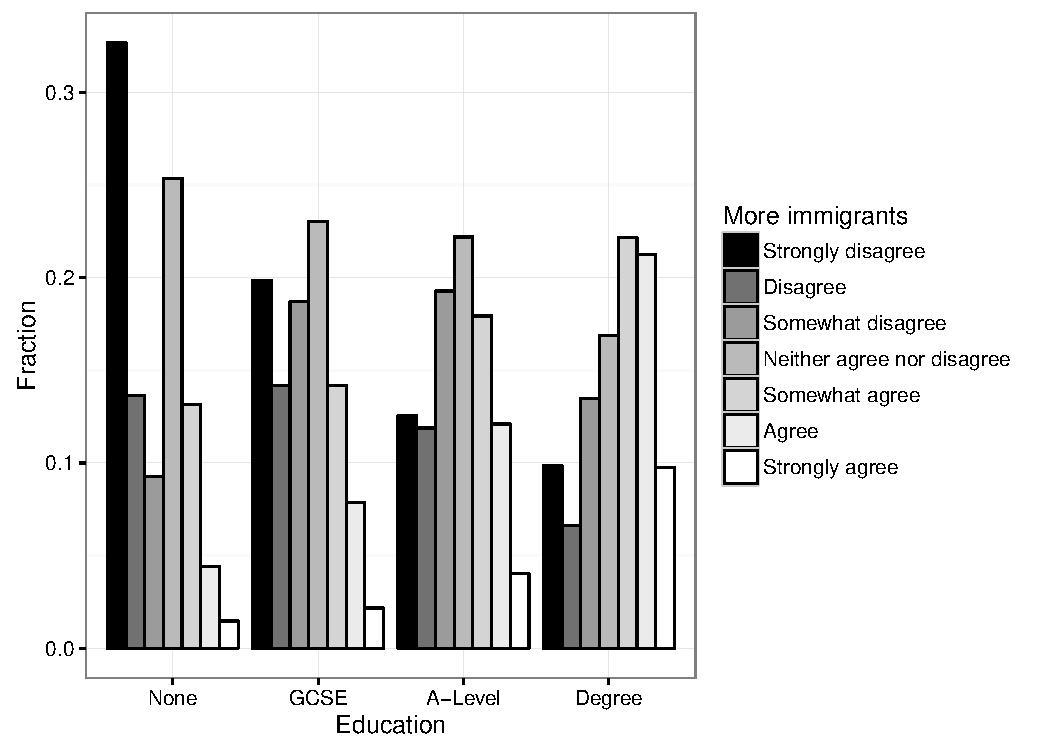
\includegraphics[width=\maxwidth]{figure/hhFig1-1} \caption[Bivariate relationship between education and anti-immigrant responses in the experiment (excludes own job experimental group)]{Bivariate relationship between education and anti-immigrant responses in the experiment (excludes own job experimental group)}\label{fig:hhFig1}
\end{figure}



Figure \ref{fig:hhFig2} shows the relationship between high and low skilled immigrants in the control group. Once again the results confirm previous findings that respondents tend to prefer high over low skilled immigrants. 

\begin{figure}
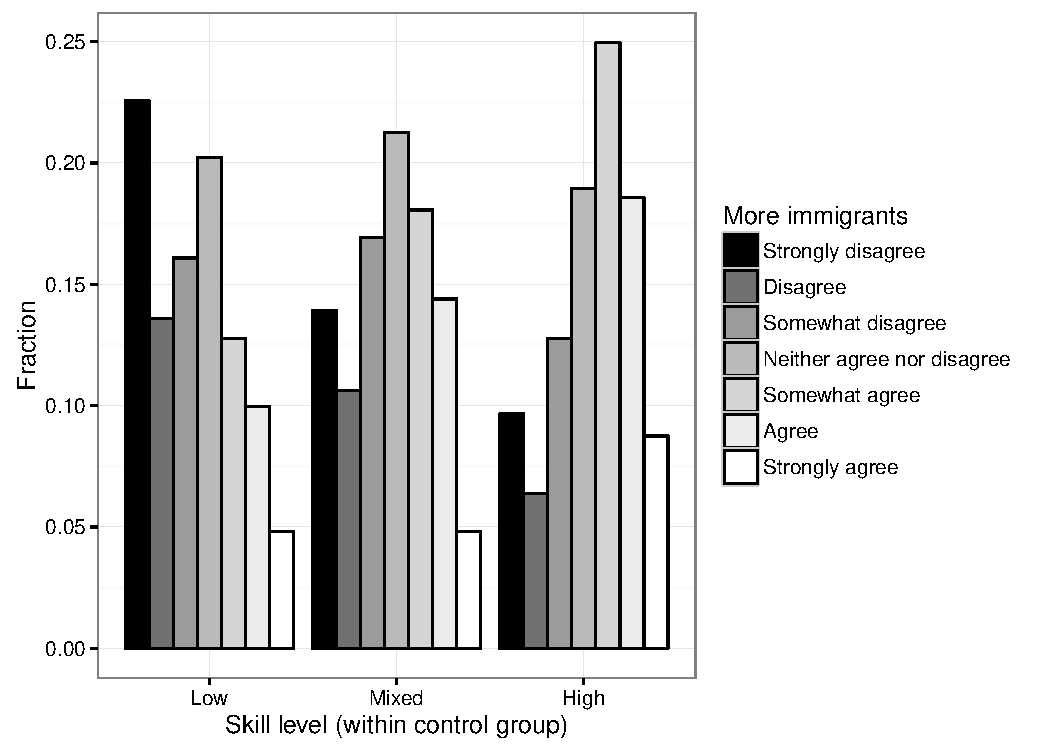
\includegraphics[width=\maxwidth]{figure/hhFig2-1} \caption[Control group support for more immigrants by skill level of immigrants  (excludes own job experimental group)]{Control group support for more immigrants by skill level of immigrants  (excludes own job experimental group)}\label{fig:hhFig2}
\end{figure}

\begin{table}

\caption{Level of concern about their own job for respondents in own job group and other groups}
\begin{tabular}{r|r}
\hline
Control groups & Own-job Treatment\\
\hline
37.1 & 33.6\\
\hline
12.6 & 10.9\\
\hline
8.0 & 7.1\\
\hline
13.2 & 14.3\\
\hline
9.6 & 9.2\\
\hline
6.8 & 9.7\\
\hline
12.6 & 15.3\\
\hline
\end{tabular}
\end{table}



\section{Experiment syntax} 
\label{appendix:experimentsyntax}

\begin{verbatim}

[immigExpDV]{single} 
Professors at several leading universities have said 
that Britain's economy could be greatly improved if 
more people were allowed to immigrate to Britain for
jobs including $Job1 and $Job2. Do you agree that 
*more* people like this should be allowed to *come
to Britain* to live and work?
<7> Strongly agree
<6> Agree
<5> Somewhat agree
<4> Neither agree nor disagree
<3> Somewhat disagree
<2> Disagree
<1> Strongly disagree
<99> Don't know


[immigExpManipCheck]{scale 1 7 dk = 1 dk_text="Don't know"}
How worried would you be about *your job prospects* if  immigrants 
like these were allowed to come to Britain in greater numbers?
-[immigManipCheck] Not at all worried | Very worried

[immigExpManipCheck2]{scale 1 7 dk = 1 dk_text="Don't know"} 
How worried would you be about immigrants like these fitting into British society?
-[immigManipCheck2] Not at all worried | Very worried

\end{verbatim}


\section{Manipulation Check Survey Screens}  \label{app:manipCheckScreens}

This appendix shows the survey screens that respondents are shown for the manipulation checks. Figure \ref{econ_threat_screen} shows the economic threat measure and figure \ref{culture_threat_screen} shows the cultural threat measure.

\begin{figure}

\includegraphics[width=10cm]{figure/econ_threat.png}
\caption{Survey screen for cultural threat that respondent sees in the experiment.}
\label{econ_threat_screen}
\end{figure}


\begin{figure}

\includegraphics[width=10cm]{figure/culture_threat.png}
\caption{Survey screen for cultural threat that respondent sees in the experiment.}
\label{culture_threat_screen}
\end{figure}

\section{Don't know responses}
The British Election Study has a policy of including don't know response options in almost all questions in order to avoid eliciting non-opinions and increase respondent retention. Don't know responses were dropped from the analysis in this study. Note that dealing with don't knows was not explicitly mentioned in the pre-analysis plan. 

This could present a potential problem if one of the treatments greatly affects the propensity to give don't know as a response. To check this, I ran a logistic regression on don't know responses using the experimental groups as predictors. Table \ref{table:dk.pred} shows the results of this analysis, which do not show any significant effects, showing that there is no systematic difference in item non-response between treatment groups. In total, 8.8\% of respondents gave a don't know response. This is reasonably in line with itme non-response on the British Election Study more generally. 


\begin{table}
\begin{center}
\begin{tabular}{l c }
\hline
 & Model 1 \\
\hline
(Intercept)              & $0.10^{***}$ \\
                         & $(0.01)$     \\
Treatment: high/ own job & $-0.01$      \\
                         & $(0.01)$     \\
Treatment: both low      & $-0.02$      \\
                         & $(0.02)$     \\
Treatment: low/ own job  & $-0.02$      \\
                         & $(0.01)$     \\
Treatment: low/high      & $-0.01$      \\
                         & $(0.01)$     \\
\hline
AIC                      & 1524.53      \\
BIC                      & 1563.48      \\
Log Likelihood           & -756.26      \\
Deviance                 & 389.43       \\
Num. obs.                & 4878         \\
\hline
\multicolumn{2}{l}{\scriptsize{$^{***}p<0.001$, $^{**}p<0.01$, $^*p<0.05$}}
\end{tabular}
\caption{Logistic regression of reporting don't know to support for immigration across experimental groups}
\label{table:dk.pred}
\end{center}
\end{table}


\end{appendix}

\end{document}
